\subsection{Isosurface Extraction}\label{sec:isocontour}

\begin{figure}[t]
\centering
\subcaptionbox{\emph{by bit plane} (\sbit)}
{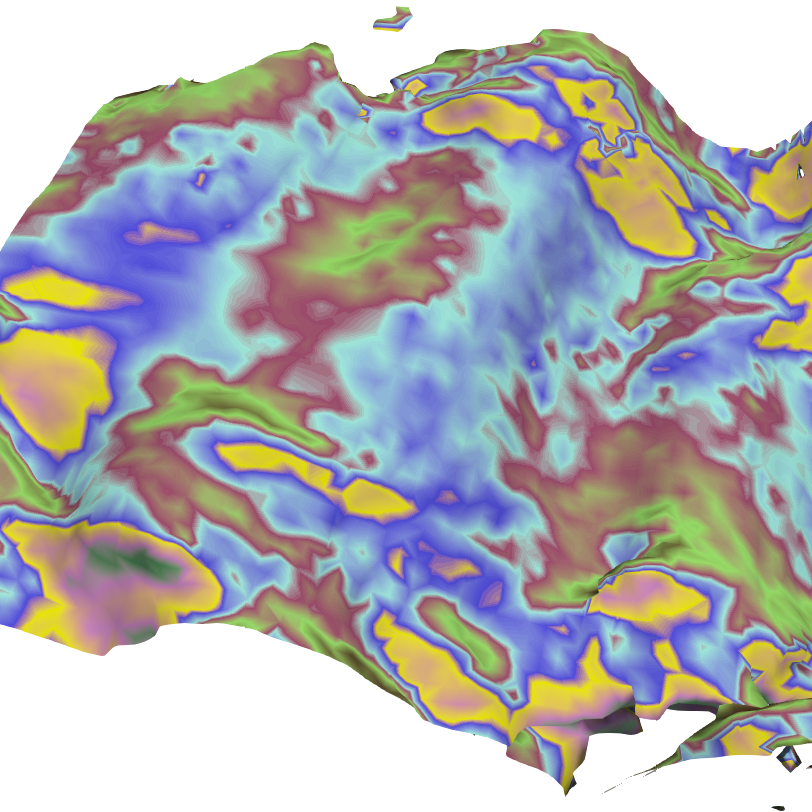
\includegraphics[width=0.32\linewidth]{isocontour/isocontour2-bit-plane}}
\subcaptionbox{\emph{by wavelet norm} (\swav)}
{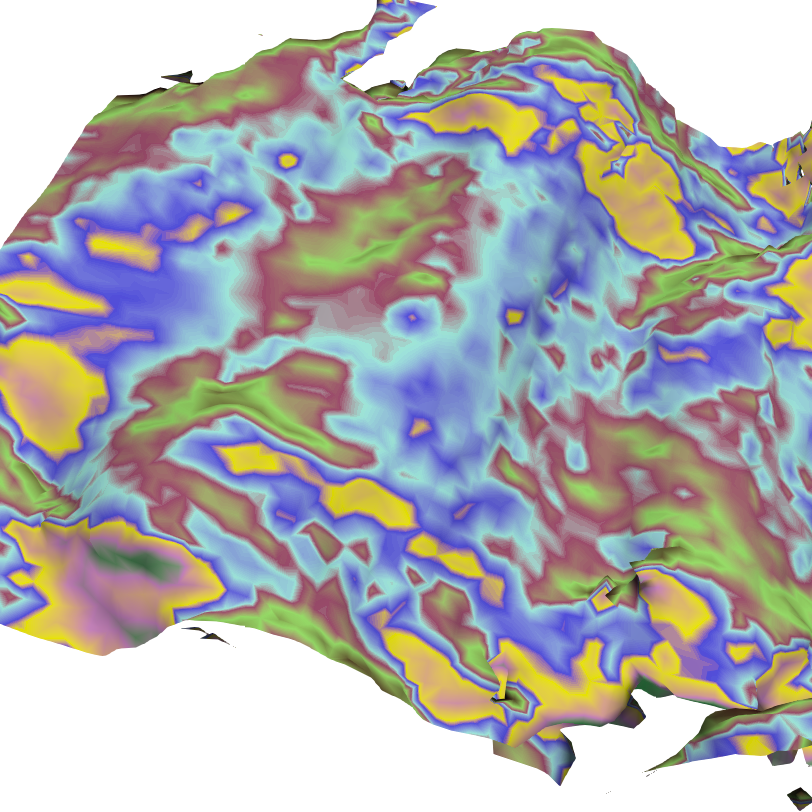
\includegraphics[width=0.32\linewidth]{isocontour/isocontour2-wavelet-norm}}
\subcaptionbox{\emph{ground truth}}
{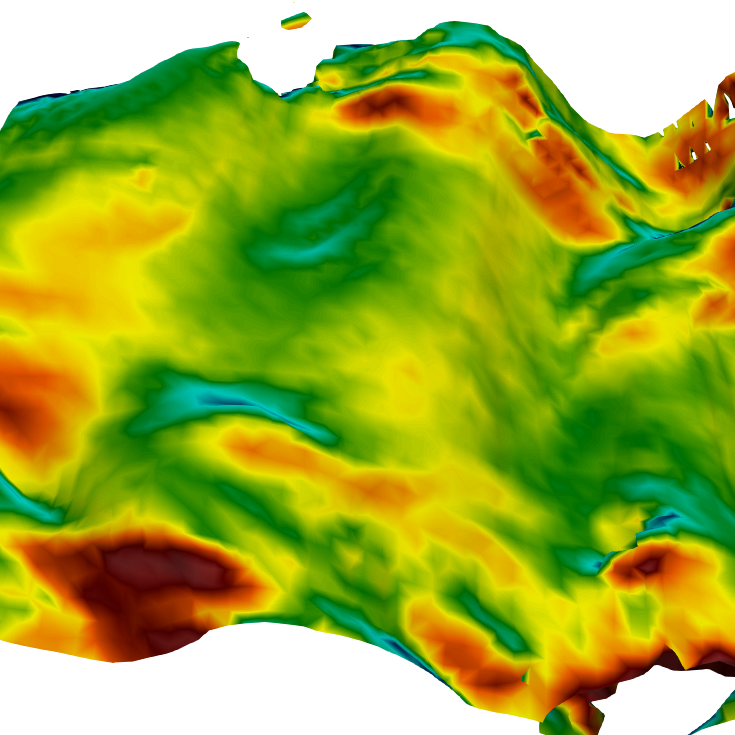
\includegraphics[width=0.32\linewidth]{isocontour/isocontour2-groundtruth}}
\caption{\emph{plasma}'s isosurface reconstructed at 0.5 bps. The surfaces are colored by the
$x$-component of the normal vectors. The reconstruction by \sbit is closer to the reference (compare
e.g., yellow features and green features).}
\label{fig:isocontour-surfaces-plasma}
\vspace{-1em}
\end{figure}

\begin{figure}[t]
\centering
 \subcaptionbox{\label{fig:bit-distrib-rmse-tile}\emph{RMSE}}{{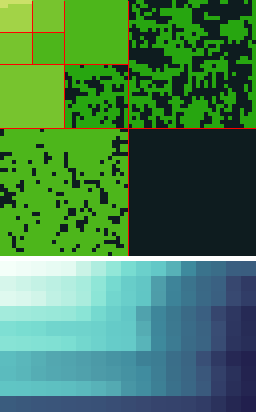
\includegraphics[width=0.32\linewidth]{bit-distrib-rmse-tile}}}
 \subcaptionbox{\label{fig:bit-distrib-laplacian-tile}\emph{Laplacian}}{{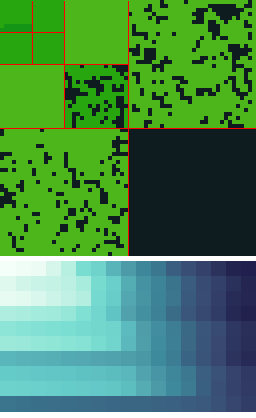
\includegraphics[width=0.32\linewidth]{bit-distrib-laplacian-tile}}}
 \subcaptionbox{\label{fig:bit-distrib-histogram-tile}\emph{histogram}}{ {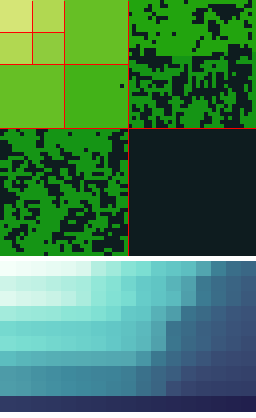
\includegraphics[width=0.32\linewidth]{bit-distrib-histogram-tile}}}
\caption{(Top) Bit distribution across subbands at 1.9 bps for signature-based streams, and (bottom)
corresponding stream signatures. The data is a 2D slice from \emph{diffusivity}. Subbands are
separated by red lines. The color of each pixel indicates the bit plane at which the corresponding
coefficient is currently at. Brighter greens correspond to more precision. Both the top and the
bottom rows show that \shsg allocates more bits to the lower subbands, while \slsg prefers to stream
bits from higher subbands. \srsg is somewhere in the middle.}
\label{fig:bit-distrib}
\vspace{-1em}
\end{figure}

Studying isosurfaces of a given function is an essential task in many visualization and analysis
pipelines, as they can highlight features of interest. For measuring error between isosurfaces, we
have found that the commonly used Hausdorff distance does not work well in our case, as two very
different reconstructed surfaces may share the same Hausdorff distance to the reference. More
sophisticated metrics exist, focusing on different characteristics such as
geometric~\cite{verifiable-isosurface} and topological~\cite{topology-verification-isosurface}
properties, but they assume the surface has certain properties. Since isosurfaces partition the
domain into ``inside'' and ``outside'' regions, we opt for a simpler error metric that assumes
nothing about the shape of the isosurfaces, but simply counts misclassified voxels. This metric
differs from comparing histograms with two bins in that we care about the spatial position and not
just voxel counts.

However, if the error caused by discarding a packet is of subvoxel resolution, such a metric fails
to capture the importance of that packet, causing \siop to be ineffective. Therefore, we add the
relative difference in surface areas ($|A_1-A_2|/|A_1|$) to the error term. This additional term is
often between $[0, 1]$, and is meant to capture the subvoxel error, when the number of misclassified
voxels is zero.

With the error metric defined, we can compute a data-dependent stream optimized for this metric
(\siop) and a stream based on its signature (\sisg) using~\Cref{alg:greedy}
and~\Cref{alg:signature}. \Cref{fig:isocontour-plots} compares the performances of these two
streams, along with \sbit, \slvl, \swav, and \smag. As can be observed, \slvl performs poorly,
indicating that isosurface extraction favors resolution over precision. \emph{plasma} is the only
data set where \sbit outperforms \swav.

For \emph{plasma}, the isosurface is extracted from a region with a low gradient, which means the
surface is very sensitive to low-ordered bits (i.e., a slight change in values moves the isosurface
by a larger distance). For this reason, \swav initially performs better (below 0.2 bps), as it
streams more precision bits. As \sbit acquires enough precision, however, it starts to resolve the
fine-scale geometry of the surface better than \swav
(from~\Cref{fig:bit-plane-vs-wavelet-norm-gradient} in~\Cref{sec:gradient}, we learn that \swav
tends to reconstruct a smoother function everywhere).

\Cref{fig:isocontour-surfaces-plasma} shows the surfaces reconstructed by \sbit
and \swav at 0.5 bps, which confirm that \sbit is able to preserve better the fine-scale surface
features. For the \emph{turbulence} field, the isosurface is extracted from a high-gradient region;
thus precision bits matter less, and \sbit outperforms \swav from the beginning. \sbit also
outperforms \sisg in this case, most likely because local signatures coming from regions that the
isosurface does not intersect can dilute those coming from regions that it does. This phenomenon
makes the signature less useful for tasks that involve localization in the spatial domain, such as
isosurface extraction. Here, it happens in various degrees for every data set but it is especially
relevant in the case of \emph{turbulence}, since the surface is confined to very small regions of
the whole volume.

For a typical isosurface that is relatively smooth and is not confined to small regions, such as
\emph{pressure} with an isovalue of 0.2, \swav typically outperforms \sbit
(see~\Cref{fig:isocontour-surfaces-pressure}). This figure renders the isosurfaces reconstructed at
0.7 bps for all streams. In terms of the quality of the reconstructed surfaces, $\sisg \approx \swav
> \sbit > \smag > \slvl$, which agrees with the curves in~\Cref{fig:isocontour-plots}. For
isosurface extraction, \swav seems to be the only stream --- among the data-independent ones ---
that consistently works well in all cases.
